% Chapter 5
%----------------------------------------------------------------------------------------
\section{Extracting the data}
\label{extracting}
\subsection{Gateway requirements}
The gateway consists of a XBee radio connected to a computer via RS232. This computer runs a separate gateway program which will be explained in this section. The computer will evolve into an embedded Linux device such as the Raspberry Pi\defcitealias{RASPBERRY}{The Raspberry Pi Foundation, 2011}\citepalias{RASPBERRY}.\\
It is important that it runs on Linux since some libraries are necessary and the serial communication is based on system calls to the Linux kernel. For instance, xerces 3.1.1\defcitealias{XER}{Xerces developers, 2010}\citepalias{XER} library for XML parsing or boost 1.49\defcitealias{BOOST}{Boost developers, 2013}\citepalias{BOOST} for multi-threading and some other small features.\\
The library for the web server is Mongoose and the one for the SQL database is SQLite\defcitealias{SQ}{QSLite developers, 2013}\citepalias{SQ}. Both libraries are written in C and consist out of a limited amount of files and are both compiled into the final program. So unlike Xerces and Boost the OS will not need to install these libraries since they are not dynamically linked.\\
RS232 is a simple serial protocol that is used for low data rates. In Linux an RS232 connection is easily set up by opening a file descriptor with the necessary options to configure baud rate, parity, stop bits, etc\citep{SWEET}. After setting up the connection read and write functions can be used to receive and to send packets to and from the XBee ZigBee radio.

\subsection{Programming language choice}
Before starting to program, a few decisions had to been made: which programming language and which operating system? One of the requirements was that the program could run on an embedded device. Linux has more options in the embedded domain than windows. For instance Raspbian, which is optimized for Raspberry Pi \defcitealias{RASP}{Raspbian developers, 2013}\citepalias{RASP}. The Raspberry Pi is a cheap embedded device with an Ethernet connection, 2 USB ports, a 700mhz ARM processor and which can run different Linux distributions.\\
The gateway program has also been tested on a Raspberry Pi running Raspbian. Going from a normal PC to a Raspberry Pi is really easy and was done without any major issues.\\
As programming language we chose for C++ since we have some experience in this programming language and it has some libraries which are not available in C. C++ also facilitates developing for example because of the built in types like String. The objects and classes allow for easier structuring of the program.

%-------------------------------------------------------------------
\subsection{Gateway program}%Implementation aspects}
\subsubsection{Overall Program Structure}
For the gateway it took some time to come up with an optimal program structure\footnote{The entire UML-diagram and code of this program can be found on Github at: \url{https://github.com/Silverslide/Qt_ZigbeeWSN}}. Since a gateway generally has to wait a lot for incoming messages on different connections, it is logical to construct threads which can wait while other threads keep on running.\\
One option would be to use the \textit{pipeline pattern} where one thread 'generates' packets. This would be the ZigBee receiver or the web service. Then a few threads would act as filters on these packets, doing the necessary processing. The last thread would be Ipsum to send data out. However, one simple pipe would not work since there are more threads generating packets. The web service as well as the ZigBee sender are generating packets. There is not really one flow of information going from one place to another. Information is coming in at different places and is also leaving the program at different places. The web service is not only generating packets, it also needs to be able to receive replies from the main thread. Ipsum on the other hand will most often receive packets but there are scenarios in which the Ipsum thread sends some packets to the main thread.\\ 
A more flexible pattern is the \textit{thread pool pattern}. This pattern is often used for web servers where each thread handles an incoming connection. This is not entirely the same for the gateway program. The gateway has a few threads, one for each type of connection. These threads are all different, whereas on a web server these threads are mostly copies of the same code. The gateway consists of a main thread that receives packets from different threads and sends out other packets. It sends these packets to different threads which handle the input and output of the gateway. Figure \ref{fig:threads} displays this structure. The transfer of packets between threads happens via queues which are protected by mutexes. These queues contain objects of a child class of Packet. All the different packets can be found in the UML on github. Since this is a gateway for ZigBee and ZigBee itself is not supposed to deal with large amounts of data, no special priorities have been set to different threads nor have the queues been limited in size or have any possible bottlenecks(they shouldn't exist) been analysed. The only optimization for multithreading that has been done, is using local queues to store packets before they are processed. So the pointers to the packets from the shared queues are copied to the local queues. Then processing is done on the packets found in these local queues. Now the shared queues are only being read while the packet pointers are being copied and not while the packets are being processed. So other threads will have to wait less for these shared queues.\\
The IO-threads in charge of dealing with correct processing of incoming and outgoing information, are: Ipsum, ZBSender, ZBReceiver and Webservice. They will be discussed in the next subsections.
\begin{figure}[t]
\centering
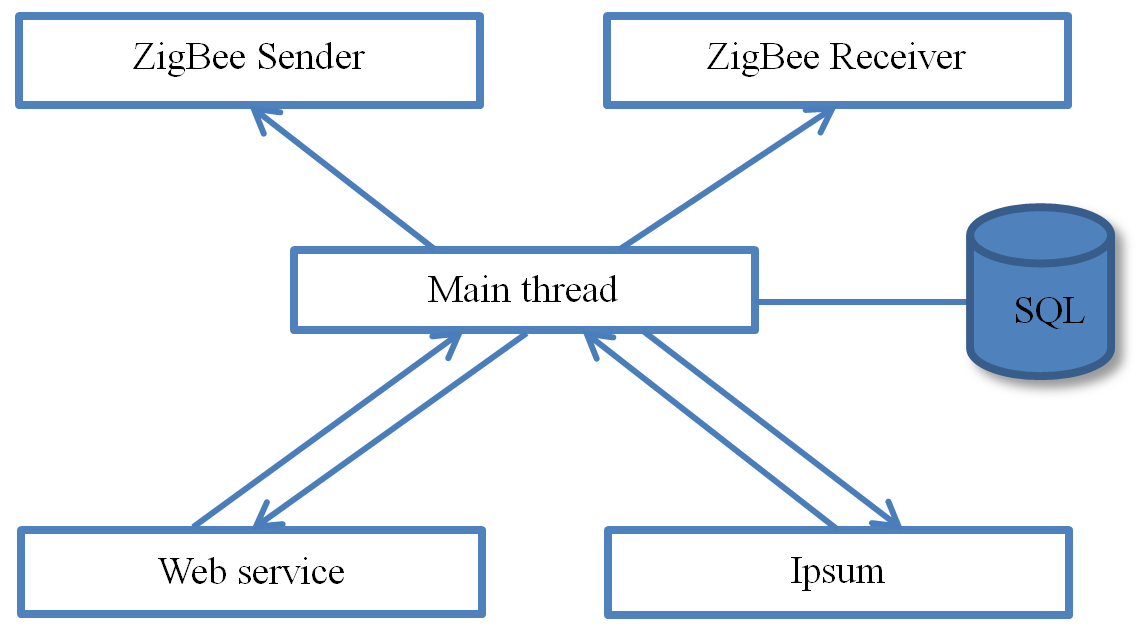
\includegraphics[width=0.48\textwidth]{threads}
\caption{Gateway thread pool model}
\label{fig:threads}
\end{figure} 
%---------------------------------
\subsubsection{IO-threads}
\paragraph{ZigBee}
On the ZigBee side there are 2 threads, one for sending packets and one for receiving packets. Received packets are pushed onto a queue that is read out in the main thread. Received packets can be sensor data, errors and responses from sent packets. Again all different packets can be found in the UML on github. When the main thread needs something to be done in the ZigBee network it will push a packet onto the queue going to the ZigBee sender thread. For instance: change sensor sample frequencies, request IO data, activate a node.
%---------------------------------

\paragraph{Ipsum}
Ipsum is the name of a storage system developed by Group T. In the gateway the Ipsum thread is thus responsible for sending data to this storage system. To do so it uses a HTTP connection and POST or GET messages where the data consist of XML \defcitealias{IPSUM}{Tacq, 2013}\citepalias{RASP}. Ipsum differs from other storage systems. It has virtual sensors to which data can be uploaded. Sensors can be grouped into sensor groups and those in can turn be grouped into installations. Figure \ref{fig:ips} shows Ipsum's internal layout. For a WSN this is exactly the structure needed. A node has different sensors so a node can be mapped on a sensor group in Ipsum. For each 'floor' in Group T a different installation is used. All these structures in Ipsum are generated by the web application. A sensor also has an 'InUse' and a 'Frequency' field by default. 'InUse' will be set to true when the ZigBee network confirmed that a sensor has been added successfully. The 'Frequency' field is actually the interval in seconds between measurements. Also a sensor group has an 'InUse' field this is also enabled when a node is successfully added.\\
\begin{figure}[t]
\centering
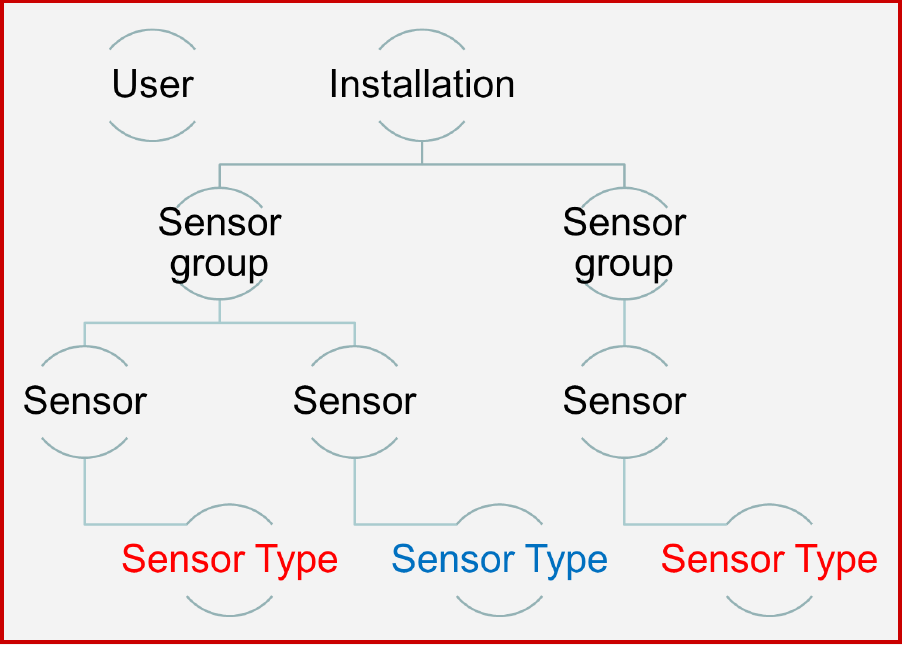
\includegraphics[width=0.48\textwidth]{ipsum}
\caption{The hierarchical design of Ipsum}
\label{fig:ips}
\end{figure} 
\noindent
Since Ipsum is a remote storage system it must be taken into account that the connection to Ipsum or Ipsum itself, can fail. Therefore local caching in the Ipsum thread is done. When Ipsum is available again all cached packets are sent out.\\
An improvement can be to check the available memory. In case memory is almost full the packets should be sent back to the main thread and stored there in the SQL database. Or a separate SQL database can be used so that the Ipsum thread can do this storage itself.

%---------------------------------
\paragraph{Web service}
The web service is a simple REST\footnote{Representational State Transfer (REST)} service which makes use of the Mongoose library. Mongoose sets up some threads (by default 20) to handle incoming connections \defcitealias{MONG}{Valenok, 2013}\citepalias{MONG}. These threads wait for incoming HTTP requests. The type of command can be found in the URL and the necessary data can be found in the POST data and is formatted in XML. The XML is read in one of the web service threads and if nothing goes wrong a HTTP 202:Accepted, is sent back to the client. If the command does not exist or the XML is invalid an error is replied. Also a key has to be added to the URL to allow for some sort of authentication. Since the key shouldn't be read by anyone or its use would be futile, the messages are encrypted using SSL. So in fact the web service uses HTTPS instead of HTTP.\\
Possible commands are: add node\footnote{This is the 'ADD\_NODE\_REQUEST' packet mentioned in section \ref{initial}.}, add sensor, request IO and change frequency. For a complete list and a detailed format of these requests please see appendix \ref{xml}.

%---------------------------------
\subsubsection{Main thread}
All intelligence can be found in the main thread. This is where the decisions are made. What to do with incoming packets? Most often this means creating new packets and putting them in the appropriate queues.\\
Since it is possible that packets going into the ZigBee network are not received nor responded to correctly, a list of sent packets is kept in the main thread. This is only done for packets we expect a reply from. For the 'request IO data' packet this is not the case. This packet is sent out and it is not replied to. Only the next time data is sampled for that node, also sensor data for sensors specified in the 'request IO data' packet is provided. But if an 'add node' or 'change frequency' packet does not receive a reply, it will be resent. The time used to expire and amount of resends done, can be set on startup. These replies are generated by the Waspmotes but also ZigBee can send back acknowledgements. If this acknowledgement is not successful then the remote radio will not have received the packet and also a resend can be done.\\
But delivering the packet to the remote radio is not sufficient. It's not because the remote radio received the packet that it has accepted it correctly. So therefore also a reply from the Waspmote is expected before the delivery can be assumed successful. A failed acknowledgement is usually faster than the timeout of a sent packet. But an acknowledgement alone is not sufficient. So this is why both factors are taken into account to resend packets.\\
The matching between an acknowledgement and the original sent packet is done by frame ID. This is an unsigned char given to each packet and when it differs from zero an acknowledgement will be sent. This frame ID can overflow, however this is not a problem unless so many packets are sent that there are now two packets with the same frame ID waiting for a response. Then the strategy is to take the last sent packet since it is most likely that this packet received a reply. If the number of resends and the expiration time of sent packets is low enough this scenario will almost never occur. Only admins can send 'add node' and 'change frequency' packets. So these admins should send more than 255 packets in the time equal to expiration time X number of resends. Normal values for expiration time are 10 or 15 seconds. The number of resends is usually below three. So this problem only occurs if more than 255 packets are sent in less than one minute.\\
The main thread also has access to local storage in the form of an SQLite database. Node information has to be stored locally in order to link ZigBee addresses to the correct Ipsum ID’s. When a sensor data packet is received, the main needs to look up to what Ipsum sensors it has to upload this data. The relation between Ipsum ID and ZigBee address is made when the web service receives add node and add sensor requests.\\
Also errors could be logged in the database. For now errors are printed to \verb+stderr+ (standard error stream) which is coupled to a file.

%------------------------------------------------------------------
